\chapter{Background} \label{cha:background}

\section{Magnolia}

Magnolia is an experimental research language being developed \gls{bldl} at the
University of Bergen. Magnolia is designed to support a high level of abstraction
and ease of reasoning. This is achieved by \textit{concepts}, \textit{axioms} and
\textit{implementations}.

\todo{expand}

\subsection{Mathematics and Programming}

Mathematics is everywhere, and useful. It's not always easy to notice this, but
one thing that helps, is knowing the names of the concepts one encounter. One
can easily understand that knowing simple operations like addition,
multiplication, etc. is useful but for more abstract mathematics, this is
harder. An example of this is abstract algebra, which is the study of algebraic
structures, which are structures that are very common in programming. A
programmer will use these structures more often than not, knowingly or
unknowingly, and a good programmer will explicitly seek these structures out.
Using existing logic; something that other people have reasoned and verified,
makes avoiding bugs easier.

An important aspect of development, is logging. Knowing what actions have taken
place is an essential tool when hunting down bugs. A common way to structure
logs, would be composing logs, depending on when they occurred. As a concrete
example, let's say we are making a text editor, and are in the need of a logging
manager, which, among other things, should compose different log statements.
Assuming we have some type \lstinline[language=Haskell]{Log A}, where there the
type \lstinline[language=Haskell]{A}, is the result of the computation a given
function, we want to be able to compose different, related, computations. But,
importantly, the order of composition of the
\lstinline[language=Haskell]{Log A}-type matters. Representing the composition
of the \lstinline[language=Haskell]{Log A}-type as $\odot$, doing, and letting
$a, b, c$ be of type \lstinline[language=Haskell]{Log A}:
\begin{equation}
  a \odot \left ( b \odot c \right ) = \left ( a \odot b \right ) \odot c
\end{equation}

Moving on, a good feature of a text editor, is being able to undo and redo
actions. These are the actions that a user can do:

\begin{itemize}
  \item Insert text at a position
  \item Delete text from a position
  \item Redo an action
  \item Undo an action
\end{itemize}

Same as in the logging example, composing is a reasonable thing to implement,
and should result in another action. Similarly, the order matters; deleting text
and then inserting, is not the same as inserting and then deleting. But we want
the \textit{inverse} of an action, so for every action we want an opposite
action that undos an action. Then our composition of actions looks different.
Say, $a$ is some action, and $c$ is some opposite action, then our composition
looks like this:

\begin{equation}
  a \odot c = U
\end{equation}

Where $U$ is an action representing \textit{no-operation}. This could be
inserting the empty string at any position, deleting the empty string at any
position, or redoing or undoing any of the aforementioned actions.

Both of these examples are relatively easy to implement, but harder to verify,
that they work correctly; that the \textit{logic} holds. But both of these two
examples are well known in mathematics, especially in \textit{Abstract Algebra}

\subsection{Abstract Algebra}

Both the logging example, and the text editor example, are some binary
operation over some set. In the first example, our set was all different log
statements of the type \lstinline[language=Haskell]{Log A}, and composing these
logs, gave us another \lstinline[language=Haskell]{Log A} type. While in the
second example, we were working on the set of actions, which we could compose,
which also gave us another action, but we also had an action representing
no-operation, and an \textit{inverse} operation, undoing an action.

In the first example, we are working with a \textit{semigroup}, and in the
second example, we are working with a \textit{group}. These are known as
algebraic structures, which is just some set, with a binary operation, and some
property on that binary operation. The trivial example, is known as
\textit{magma}, and is defined by \ref{def:magma}. The closure \ref{def:closed}
simply specifies that we only work with one set.

\begin{definition}[Closure] \label{def:closed}
  For a set $M$, with a binary operation $\oplus$,
  $\forall a, \forall b, \exists c \in M$, such that
  $a \oplus b = c$.
\end{definition}

\begin{definition}[Magma] \label{def:magma}
  A magma is a set $M$, with a binary operation $\oplus$, which is
  \ref{def:closed}
\end{definition}

We can \textit{extend} the definition of magma, by adding associativity on the
binary operation. This \ref{def:assoc}, as shown in the examples, simply
specifies that the order we evaluate our composition matters.

\begin{definition}[Associtativity Law] \label{def:assoc}
  For any binary operation $\oplus$, on a set $M$, $a, b, c \in M$.
  $a \oplus \left ( b \oplus c \right ) = \left ( a \oplus b \right ) \oplus c$,
  must hold.
\end{definition}

This associativity gives us a semigroup, as shown in the definition
\ref{def:semi}, which is the structure that we modeled in our logging example.

\begin{definition}[Semigroup] \label{def:semi}
  A semigroup is a set $M$, with a binary operation $\oplus$, and $\oplus$ must
  uphold \ref{def:closed} and \ref{def:assoc}.
\end{definition}

By simply adding the identity law (\ref{def:ident}), we get a
monoid (\ref{def:monoid}), and adding the inverse law
(\ref{def:inv}), we get a group.

\begin{definition}[Identity Law] \label{def:ident}
  For any binary operation $\oplus$, on a set $M$,
  $\forall a, \exists U \in M$, such that
  $a \oplus U = a$, and $U$ is unique.
\end{definition}

\begin{definition}[Monoid] \label{def:monoid}
  A monoid is a set $M$, with a binary operation $\oplus$, and $\oplus$ must
  uphold \ref{def:closed}, \ref{def:assoc} and \ref{def:ident}.
\end{definition}

\begin{definition}[Inverse Law] \label{def:inv}
  For any binary operation $\oplus$, on a set $M$,
  $\forall a, \exists U \in M$, such that
  $a \oplus U = a$, and $U$ is unique.
  And $\forall a, \exists b \in M$, such that $a \oplus b = U$, and the mapping
  for $a \to b$ is one-to-one.
\end{definition}

\begin{definition}[Group] \label{def:group}
  A group is a set $M$, with a binary operation $\oplus$, and $\oplus$ must
  uphold \ref{def:closed}, \ref{def:assoc}, \ref{def:ident} and \ref{def:inv}.
\end{definition}

This definition \ref{def:group}, of course is identical to the structure we used
to model undo-redo, in our text editor example. To avoid common mistakes when
implementing these structures, it would behoove a developer if they could encode
these properties in something like an interface or type class, like in Java.

\subsection{Java Group}

This structure not could be implemented in something like Java, an
Object-Oriented Language, as shown in listings \ref{lst:jmagma},
\ref{lst:jsemigroup}, \ref{lst:jmonoid}, and \ref{lst:jgroup}. Note the empty
interfaces; there is nothing that enforces the different laws on the properties.
This can only be done by unit testing, which is not enforced on a consumer of
the \gls{api}.

\begin{center}
  \lstinputlisting
    [ language=Java
    , caption={Magma concept in Java}
    , label=lst:jmagma]{./code/magma.java}
\end{center}

\begin{center}
  \lstinputlisting
    [ language=Java
    , caption={Semigroup concept in Java, can only be upheld using unit tests}
    , label=lst:jsemigroup]{./code/semigroup.java}
\end{center}

\begin{center}
  \lstinputlisting
    [ language=Java
    , caption={Monoid concept in Java, can only be upheld using unit tests}
    , label=lst:jmonoid]{./code/monoid.java}
\end{center}

\begin{center}
  \lstinputlisting
    [ language=Java
    , caption={Group concept in Java, can only be upheld using unit tests}
    , label=lst:jgroup]{./code/group.java}
\end{center}


\subsection{Haskell Group}

This can also not be implemented in Haskell. Using typeclasses, one cannot
enforce properties on the defined methods. Again, notice the empty extensions
in listing \ref{lst:hsemigroup} and \ref{lst:hgroup}.

\begin{center}
  \lstinputlisting
    [ language=Haskell
    , caption={Magma concept in Haskell}
    , label=lst:hmagma]{./code/magma.hs}
\end{center}

\begin{center}
  \lstinputlisting
    [ language=Haskell
    , caption={Semigroup concept in Haskell, can only be upheld using unit tests}
    , label=lst:hsemigroup]{./code/semigroup.hs}
\end{center}

\begin{center}
  \lstinputlisting
    [ language=Haskell
    , caption={Monoid concept in Haskell, can only be upheld using unit tests}
    , label=lst:hmonoid]{./code/monoid.hs}
\end{center}

\begin{center}
  \lstinputlisting
    [ language=Haskell
    , caption={Group concept in Haskell, can only be upheld using unit tests}
    , label=lst:hgroup]{./code/group.hs}
\end{center}

\subsection{Magnolia Group}

In Magnolia, however, this can be enforced on the \textit{interface}-level. The
example code shown in listing \ref{lst:magma}, showcases a concept
representation a binary operation, which has one function, \textit{binop}, which
takes in two values of type \textit{T}, and returns \textit{T}. Note that the
actual implementation of this function is missing. This is because a concept
encodes the properties of a users code. The actual implementation of the
binary function needs to uphold the properties of the concept that is
being implemented. Note that this is unlike the Java and Haskell example, in
which we have no way to encode the property of our binary function. So any
consumer of our \gls{api} would not be explicitly bound to our restriction of
the associativity law \ref{def:assoc}, identify law \ref{def:ident}, and the
inverse law \ref{def:inv}, required by semigroup and group. The closure
definition, \ref{def:closed}, however, can be encoded by the type system in Java
and Haskell.

\begin{center}
  \lstinputlisting
    [ language=Magnolia
    , caption={Magma concept in Magnolia}
    , label=lst:magma]{./code/magma.mg}
\end{center}

In the example code shown in listing \ref{lst:semigroup}, the \textit{magma}
concept has been expanded upon, still following the same rules as before, but
with the added property of associativity.

\begin{center}
  \lstinputlisting
    [ language=Magnolia
    , caption={Semigroup concept in Magnolia}
    , label=lst:semigroup]{./code/semigroup.mg}
\end{center}

\begin{center}
  \lstinputlisting
    [ language=Magnolia
    , caption={Monoid concept in Magnolia}
    , label=lst:monoid]{./code/monoid.mg}
\end{center}

\begin{center}
  \lstinputlisting
    [ language=Magnolia
    , caption={Group concept in Magnolia}
    , label=lst:group]{./code/group.mg}
\end{center}

So Magnolia facilitates reuse, and extension of logic. \todo{expand}

\section{Reusable Software}

One of the most important features in any programming language, is the notion
of \textit{reusability}. From the invention of the GO-TO-statement,
to functions, and external libraries, being able to reuse existing software is
an important tool for a developer. It avoids \textit{re-inventing the wheel}, as
common functionality can be externalized and reused in several different places.

\subsection{Reuse in Magnolia}

Reusability is also an important feature in Magnolia, but this reusability is in
the entire language. In libraries in other languages, functions are reused, in
an attempt to avoid common logical mistakes, but these mistakes could still be
there, hiding in plain view. In Magnolia, one can re-use the \textit{logic} of a
function. The logging and group example can be written using Magnolia concepts
as shown in listing \ref{lst:logging} and \ref{lst:editor} respectively.

\begin{center}
  \lstinputlisting
    [ language=Magnolia
    , caption={Logging example}
    , label=lst:logging]{./code/logging.mg}
\end{center}

\begin{center}
  \lstinputlisting
    [ language=Magnolia
    , caption={Editor example}
    , label=lst:editor]{./code/editor.mg}
\end{center}

\subsection{Software Lifetimes}

Software in general, lasts around 30 years (source). This is quite a long time,
but, this statistic is about more \textit{rigid} applications, which have an
unchanging scope. In more \textit{chaotic} fields, this number is reduced, as
paradigm shifts within certain fields, which results in the need for drastic
changes in the existing applications, where the needed work to change the code,
can be more than to create a new application.

\subsection{Software Longevity}

Most examples of \textit{popular} software, are open source, like \gls{vim}.
\gls{vim} is a text editor which has been in use since 1991. There are several
factors behind this success, but the ones being highlighted here, are due to its
extensibility and due to it being open-sourced. Being open sourced, allows for a
rotating cast of maintainers, ensuring the core application has the features its
users wants. The users of \gls{vim} can be split into two categories,
\textit{standard users}, and \textit{module developers}. \gls{vim} has an
extensive module ecosystem, which can extend \gls{vim}s functionality from a
text editor, to a fully fledged \gls{ide}.

\section{Integrated Development Environment} \label{sec:ide}

An \gls{ide}, aids a developer, as all the needed tools for development are
integrated into one application. There are two different kinds of \gls{ide}s,
generic and specialized. \todo{Source}

A specialized \gls{ide} is one targeted towards a specific language, like
Eclipse, (reference?), or IntelliJ (reference?), which target Java/JVM. It
contains specialized features like the following:

\paragraph{Syntax Highlighting} Highlighting important keywords, identifiers
and more, makes the language easier to read for the developer, allowing them to
spot easy to miss errors, like misspelling of keywords.

\paragraph{Code Autocompletion} Suggesting keywords, method names or even entire
code snippets, is a powerful tool an \gls{ide} can have. This is possible to
achieve, in some form, without being specialized, by for example, suggesting
text that already exist in the document, but is most useful if it is
specialized, and can suggest built-in methods. This allows a developer to not
having to remember exactly how methods are named, is the method to split a
string by some delimiter, \textit{split\_by} or \textit{split\_on}? As long as
the developer writes \textit{split}, the correct method name will be suggested.

\paragraph{Go-To-Definitions} Being able to quickly navigate to methods and read
their implementation is a useful tool for a developer, as less time has to be
spent navigating the project structure, to figure out where some method was
implemented, and more time can be spent actually developing.

A lot of these features are possible due to \textit{Language Server Protocols},
which allow for a standardized way for compilers to give code-support to
\gls{ide}'s.

A generic \gls{ide} contains the features that are common among development in
any programming language, like:

\paragraph{File Explorer} Most project nowadays is larger than one file, so
being able to visualize the project in a tree-like-structure, and navigate that,
is useful. This feature usually comes with the ability to manipulate the project
structure, by adding files, folders, moving files around, and deleting them.

But creating any \gls{ide} would still limit the lifetime of the application.
The best example of a long living active \gls{ide}, or, at least editor, is Vim
(source?). Vim is not a feature full editor, but it is simple, lightweight, and
works on any operating system. But most people use it, for how easy it is to
extend; Its lifetime has been greatly extended by the ease of modularization.
Any popular module for Vim is open-source, and therefore, if any module had an
active community around it, if the \textit{lead} developer of the module stopped
developing it, that community can continue to develop the module, either by
getting maintenance access to the repository, or by forking it. Ensuring the
lifetime of the module is extended.

\section{Module Architecture}

\todo{Talk about modules in IDEs}

A modular application, is an application which can be extended by other pieces
of software. This extensibility is useful as features that the original
developers of the application did not think about, can be added. If this module
architecture is well-designed, then this extension can be added without changing
the core application.

There are different methods an application can be extended. The most common one
uses so-called \textit{live-reload}, in which, if a module drastic changes the
functionality of an application, the application has to be restarted, or if it
is a \textit{minor} change, the module is simply loaded. This method is
extending of the application during runtime, which is the method most users
expect. Another method would be \textit{compile-time-extension}, in which
modules are added before the application itself is compiled. There are some
advantages and disadvantage in both approaches.

\subsection{Compile Time Extension}

\todo{Expand}
As an example, a standard user of any application will expect the application to
come bundled with all the needed functionality. This is best achieved with the
\textit{compile-time-extension} method, since the application can be installed
with the expected modules.

\subsection{Runtime Extension}

\todo{Expand}


\subsection{Module Ecosystem}

\todo{Expand}
More modules == better, right?

\subsection{Granularity}

When designing modules, the \textit{granularity} of the combined modules has to
be considered. As an example, if one where to extend the zero-core application
with the needed functionality for it to be considered an \gls{ide}, this could be
achieved by creating a singular module which does all the work. However, this
is not a modular approach, as if one wants to change some specific feature in
the \gls{ide}-module, one would have to re-create the whole module with that
specific feature implemented. Instead, if this functionality was granular,
that is to say, split into several modules, that together enable the needed
features, then it would be \textit{simpler} to modify the needed modules to
achieve the wanted feature.


\subsection{Module Family}

\begin{figure}
  \centering
  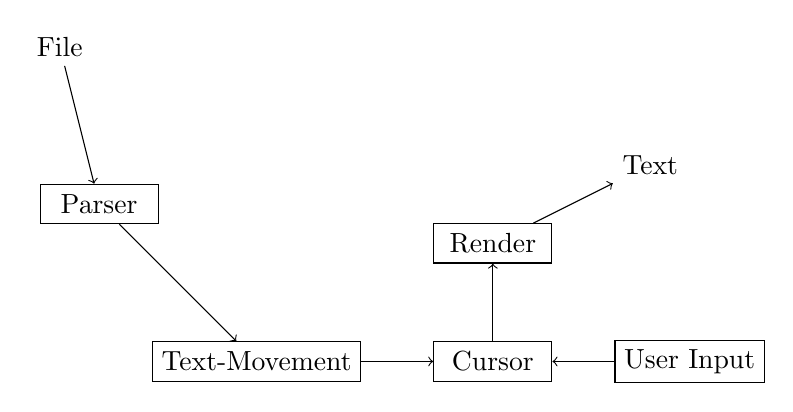
\begin{tikzpicture}
  % Nodes
  \node (file) [] at (-6, 3) {File};
  \node (parser) [rectangle, draw, minimum height=0.5cm, minimum width=1.5cm] at (-5.5, 1) {Parser};
  \node (text-movement) [rectangle, draw, minimum height=0.5cm, minimum width=1.5cm] at (-3.5, -1) {Text-Movement};
  \node (cursor) [rectangle, draw, minimum height=0.5cm, minimum width=1.5cm] at (-0.5, -1) {Cursor};
  \node (user-input) [rectangle, draw, minimum height=0.5cm, minimum width=1.5cm] at (2, -1) {User Input};
  \node (render) [rectangle, draw, minimum height=0.5cm, minimum width=1.5cm] at (-0.5, 0.5) {Render};
  \node (text) at (1.5, 1.5) {Text};
  % Arrow
  \draw[->] (file) -- (parser) node[midway, above] {};
  \draw[->] (parser) -- (text-movement) node[midway, above] {};
  \draw[<-] (cursor) -- (text-movement) node[midway, above] {};
  \draw[<-] (cursor) -- (user-input) node[midway, above] {};
  \draw[->] (cursor) -- (render) node[midway, above] {};
  \draw[->] (render) -- (text) node[midway, above] {};
\end{tikzpicture}

  \caption{Text Editor Module Family}
  \label{fig:textEditorSimple}
\end{figure}

In figure \ref{fig:textEditorSimple}, an input file is parsed to some structure
which is used to translate user actions, into cursor movements. The cursor being
the place in the file where text is written to by the user.

This is a feature that naturally shows up in a \textit{true} modular system. If
several modules together enable some feature, then those modules can be treated
as a singular module by an external module developer, depending on what they
want to extend.

\section{Language Workbench}

Language workbenches are environments for simplifying the creation and use of
computer languages. \cite{lwb}

\todo{Expand}

\section{Language Server}

The most important features in a modern \gls{ide} are possible due to the
\gls{lsp}. \gls{lsp} is a protocol for a language server and editor,
(the client), with which they communicate, allowing for many of the features
mentioned in section \ref{sec:ide}, and explicitly mentioned in table
\ref{tbl:ide}. \gls{lsp} being the standard since the 2020s, is a sign of
modularity being preferred, as now a single \gls{lsp} can be created, and used
across several different applications, like IntelliJ, VS Code and \gls{vim}.
While useful for \textit{standard} language, this is the limiting factor when it
comes to supporting experimental languages, as not only does a new set of
protocols need to be appended to a language server, the editor itself needs to
be changed to actually use these protocols. This creates a lot of work, for both
the \gls{ide} developer and for the compiler developer. Here is where a modular
approach can help both. If some new functionality or feature is added to the
experimental language, this off course means the compiler/interpreter has to be
expanded and/or modified, but for the \gls{ide}, a module could be added and/or
modified to utilize this change, instead of having to change the entire
application.

\begin{table}[]
  \centering
  \caption{IDE features enabled by LSP}
  \label{tbl:ide}
  \begin{tabular}{|l|l|}
    \hline
    IDE Feature & LS-Protocol \\ \hline
    Go to Declaration & textDocument/definition \\ \hline
    Go to Implementation & textDocument/implementation \\ \hline
    Auto-completion & textDocument/completion \\ \hline
    Hover & textDocument/hover \\ \hline
    Warnings & textDocument/publishDiagnostics \\ \hline
    Rename & textDocument/rename \\ \hline
  \end{tabular}
\end{table}

\section{Existing Magnolia IDE}

The current \gls{ide} for Magnolia \cite{baggeIde}, is a many-years-old version
of Eclipse, using modules and functionality from the core Eclipse application,
that has since been outdated. The \gls{ide}s lifetime was limited by a
dependency on external modules and features that where not maintained by the
\gls{ide}-developers. This meant that for future development of Magnolia, an
outdated \gls{ide} was needed, with outdated tooling. Furthermore, the Magnolia
compiler was implemented as an Eclipse module, which means that development is
limited to Eclipse, and only Eclipse, as a developer cannot compile Magnolia
code without it.

Modularization will help to mitigate some of the issues with the current
Magnolia \gls{ide}. Instead of maintaining an entire application, the needed and
wanted features of the application can be maintained instead.

Experimental languages might have features which are not possible to be fully
used in current \gls{ide}s. This is also the case for the current Magnolia
\gls{ide}. The compiler for Magnolia, syntax highlighting, error reporting, and
hover-functionality are functionality made in the Eclipse \gls{ide}, by using
its plug-in architecture. Some of the functionality and plug-ins this
implementation used, have been deprecated in later version of Eclipse. This
means the Magnolia \gls{ide} is locked to an old version of Eclipse, which, as
time passes, increases the complexity of installation, as the surrounding
tooling and libraries needed by this version of Eclipse also becomes deprecated.
Currently, in INF220, at the university, two weeks are set aside for students to
be able to install it.
